% In The Name of Allah
% template.tex
% Author: Amirhossein Alian

%----------------------------------------------------------------------------------------
%	LANGUAGE SWITCH
%----------------------------------------------------------------------------------------
% Persian (RTL) or English (LTR). Flip this ONE line; fonts, direction and the
% fixed labels (Outline, Questions, ...) follow it.
\newif\ifpersian
\persianfalse   % \persiantrue for a Persian presentation

%----------------------------------------------------------------------------------------
%	DOCUMENT CLASS
%----------------------------------------------------------------------------------------

\PassOptionsToPackage{table}{xcolor} % Enables \rowcolors in tables
\documentclass[
	11pt,              % 10pt--12pt read well on a projector
	aspectratio=169,   % 16:9 matches modern projectors/screens; use 43 for old 4:3 ones
	%handout,          % Uncomment to print: collapses \pause / overlays into single slides
	%t,                % Uncomment to top-align slide content (default: vertically centered)
]{beamer}

\graphicspath{{images/}{../images/}} % Slide images + the proposal's images (KUT logo)

%----------------------------------------------------------------------------------------
%	PACKAGES
%----------------------------------------------------------------------------------------

\usepackage{booktabs}  % \toprule \midrule \bottomrule
\usepackage{tabularx}  % Tables that stretch to \linewidth
\usepackage{array}
\usepackage{listings}  % Code / JSON / config snippets
\usepackage{tikz}      % Timeline and simple diagrams
\usetikzlibrary{positioning, arrows.meta, shapes.geometric}

%----------------------------------------------------------------------------------------
%	THEME: Madrid + custom palette
%----------------------------------------------------------------------------------------
% Colors match Farnama_Proposal.tex so the document and the slides look like one project.
% Want a different look? Change only `brand` and `accent` — everything else derives from them.
%   Navy / teal (default) : brand 24,46,92   accent 0,112,150
%   Dark green / green    : brand 20,70,50   accent 30,130,90
%   Burgundy / orange     : brand 110,20,40  accent 200,90,20

\usetheme{Madrid}
\useinnertheme{circles}   % Round bullets and numbered items; try `rectangles` for a sharper look

\definecolor{brand}{RGB}{24, 46, 92}       % deep navy
\definecolor{accent}{RGB}{0, 112, 150}     % teal blue
\definecolor{lightbg}{RGB}{241, 245, 251}  % block bodies, zebra rows
\definecolor{rulegray}{RGB}{190, 200, 215}
% Inline term colors (same meaning as in the proposal)
\definecolor{engblue}{RGB}{0, 86, 196}     % tools, languages, frameworks
\definecolor{engred}{RGB}{184, 28, 48}     % concepts, patterns, practices
\definecolor{engpurple}{RGB}{118, 52, 160} % standards, protocols, formats
\definecolor{enggreen}{RGB}{0, 128, 80}    % commands, file names, identifiers
\definecolor{lvlhigh}{RGB}{200, 30, 40}
\definecolor{lvlmed}{RGB}{205, 120, 0}
\definecolor{lvllow}{RGB}{0, 128, 80}

% Madrid's footline/header use palette primary/secondary/tertiary
\setbeamercolor{palette primary}{bg=brand, fg=white}
\setbeamercolor{palette secondary}{bg=brand!85!accent, fg=white}
\setbeamercolor{palette tertiary}{bg=accent, fg=white}
\setbeamercolor{palette quaternary}{bg=brand, fg=white}
\setbeamercolor{structure}{fg=brand}
\setbeamercolor{frametitle}{bg=brand, fg=white}
\setbeamercolor{framesubtitle}{fg=white!80!accent}
\setbeamercolor{title}{bg=brand, fg=white}
\setbeamercolor{item projected}{bg=accent, fg=white}
\setbeamercolor{itemize item}{fg=accent}
\setbeamercolor{itemize subitem}{fg=brand}
\setbeamercolor{alerted text}{fg=engred}
\setbeamercolor{section in toc}{fg=brand}
\setbeamercolor{subsection in toc}{fg=brand!70}
% Blocks
\setbeamercolor{block title}{bg=brand, fg=white}
\setbeamercolor{block body}{bg=lightbg, fg=black}
\setbeamercolor{block title example}{bg=enggreen, fg=white}
\setbeamercolor{block body example}{bg=enggreen!7, fg=black}
\setbeamercolor{block title alerted}{bg=lvlhigh, fg=white}
\setbeamercolor{block body alerted}{bg=lvlhigh!7, fg=black}
\setbeamertemplate{blocks}[rounded][shadow=false]

% Cleaner chrome
\setbeamertemplate{navigation symbols}{}           % Hide the PDF navigation icons
\setbeamertemplate{caption}[numbered]
\setbeamerfont{frametitle}{series=\bfseries}
\setbeamerfont{title}{series=\bfseries, size=\LARGE}
\setbeamersize{text margin left=1.2cm, text margin right=1.2cm}

% Show covered overlay items faintly instead of hiding them (comment out to hide)
%\setbeamercovered{transparent=15}

% Small logo in the top corner of every frame title
\logo{
\includegraphics[height=0.75cm]{KUT-Logo.png}\hspace{0.15cm}\vspace{-0.1cm}}

%----------------------------------------------------------------------------------------
%	FONTS & LANGUAGE (must stay after the theme)
%----------------------------------------------------------------------------------------

\ifpersian
	\usepackage{xepersian}   % Must be the last package loaded
	\settextfont[BoldFont={IRANSans Medium}]{IRANSans}
	\setlatintextfont{Open Sans}
	\setmonofont[Scale=0.9]{Source Code Pro}
	\newcommand{\eng}[1]{\lr{#1}}
	\newcommand{\txtOutline}{فهرست مطالب}
	\newcommand{\txtQuestions}{پرسش و پاسخ}
	\newcommand{\txtThanks}{با سپاس از توجه شما}
	\newcommand{\txtInstructor}{استاد درس}
	\newcommand{\txtBackup}{اسلایدهای پشتیبان}
\else
	\usepackage{fontspec}
	\setsansfont{Open Sans}
	\setmonofont[Scale=0.9]{Source Code Pro}
	\newcommand{\eng}[1]{#1}
	\newcommand{\txtOutline}{Outline}
	\newcommand{\txtQuestions}{Questions?}
	\newcommand{\txtThanks}{Thank you for your attention}
	\newcommand{\txtInstructor}{Instructor}
	\newcommand{\txtBackup}{Backup Slides}
\fi

%----------------------------------------------------------------------------------------
%	HELPER COMMANDS
%----------------------------------------------------------------------------------------

% Inline terms — one color per kind of term (same as the proposal)
\newcommand{\engb}[1]{\textcolor{engblue}{\eng{#1}}}             % tools, frameworks: \engb{Django}
\newcommand{\engr}[1]{\textcolor{engred}{\eng{#1}}}              % concepts: \engr{REST API}
\newcommand{\engp}[1]{\textcolor{engpurple}{\eng{#1}}}           % standards/formats: \engp{JSON}
\newcommand{\cmd}[1]{\textcolor{enggreen}{\eng{\texttt{#1}}}}    % code/file names: \cmd{docker compose up}
% Risk / priority levels
\newcommand{\high}[1]{\textcolor{lvlhigh}{\textbf{#1}}}
\newcommand{\med}[1]{\textcolor{lvlmed}{\textbf{#1}}}
\newcommand{\low}[1]{\textcolor{lvllow}{\textbf{#1}}}
% Emphasis without italics (italics look poor on projectors)
\renewcommand{\emph}[1]{\textcolor{accent}{\textbf{#1}}}

% Left-aligned stretching column for tabularx (plain X justifies and leaves gaps)
\newcolumntype{L}{>{\raggedright\arraybackslash}X}

% Code listings
\lstdefinelanguage{json}{
	morestring=[b]",
	literate={:}{{\textcolor{brand}{:}}}1 {,}{{\textcolor{brand}{,}}}1
	         {\{}{{\textcolor{accent}{\{}}}1 {\}}{{\textcolor{accent}{\}}}}1
	         {[}{{\textcolor{accent}{[}}}1 {]}{{\textcolor{accent}{]}}}1,
}
\lstset{
	basicstyle=\ttfamily\footnotesize,
	keywordstyle=\color{engblue}\bfseries,
	stringstyle=\color{enggreen},
	commentstyle=\color{gray}\itshape,
	backgroundcolor=\color{lightbg},
	frame=single, rulecolor=\color{rulegray}, framesep=4pt,
	breaklines=true, showstringspaces=false, columns=fullflexible,
	numbers=none, tabsize=2,
}

% Automatic section divider: shows the outline with the current section highlighted
\AtBeginSection[]{
	\begin{frame}[noframenumbering]
		\frametitle{\txtOutline}
		\tableofcontents[currentsection, hideothersubsections]
	\end{frame}
}

% Only count the main slides in "x / N" (backup slides are excluded, see the end)
\newcommand{\backupbegin}{\newcounter{finalframe}\setcounter{finalframe}{\value{framenumber}}}
\newcommand{\backupend}{\setcounter{framenumber}{\value{finalframe}}}

%----------------------------------------------------------------------------------------
%	PRESENTATION INFORMATION
%----------------------------------------------------------------------------------------
% [short] versions appear in the footline of every slide.

\title[Farnama]{Farnama}
\subtitle{Software Engineering Course Project --- Proposal Presentation}
\author[Mirzaei, Azizi, Alian]{%
	Zahra Mirzaei \and Amirmahdi Azizi \and Amirhossein Alian}
\institute[KUT]{Kermanshah University of Technology}
\date[\today]{\txtInstructor: Dr.\ Sudabeh Mohammadi \\[0.2em] \today}

% Title page layout: logo on top, then the usual Madrid title box
\titlegraphic{
\includegraphics[height=1.8cm]{KUT-Logo.png}}

%----------------------------------------------------------------------------------------

\begin{document}

%=== FRAME: Title ======================================================================
{
\setbeamertemplate{logo}{} % No corner logo on the title slide (it's already big)
\begin{frame}[plain, noframenumbering]
	\titlepage
\end{frame}
}

%=== FRAME: Outline ====================================================================
\begin{frame}{\txtOutline}
	\tableofcontents[hideallsubsections]
\end{frame}

%----------------------------------------------------------------------------------------
\section{Introduction}
%----------------------------------------------------------------------------------------

%=== FRAME: Bullet list (with step-by-step reveal) =====================================
\begin{frame}{Problem \& Motivation}
	\framesubtitle{Why does this product need to exist?}

	\begin{itemize}
		\item<1-> \textbf{Problem:} one sentence describing the pain point
		\item<2-> \textbf{Who suffers:} students, associations, university staff
		\item<3-> \textbf{Today:} how it is handled now and why that fails
			\begin{itemize}
				\item paper forms, scattered messenger groups
				\item no tracking, no history
			\end{itemize}
		\item<4-> \textbf{Our solution:} \emph{Farnama} --- one platform for all of it
	\end{itemize}
	% <n-> reveals an item on click n. Remove the <..> parts for a static slide.
\end{frame}

%=== FRAME: Blocks (definition / highlight / warning) ==================================
\begin{frame}{Product Vision}

	\begin{block}{Vision Statement}
		For \textit{target users} who \textit{need X}, Farnama is a \textit{product category}
		that \textit{key benefit}. Unlike \textit{current alternative}, our product \textit{differentiator}.
	\end{block}

	\begin{exampleblock}{In Scope}
		Association management, event requests, elections, notifications.
	\end{exampleblock}

	\begin{alertblock}{Out of Scope}
		Payments, iOS app (in this version).
	\end{alertblock}
\end{frame}

%----------------------------------------------------------------------------------------
\section{Requirements}
%----------------------------------------------------------------------------------------

%=== FRAME: Two columns ================================================================
\begin{frame}{Functional vs.\ Non-Functional Requirements}
	\begin{columns}[T] % [T] aligns column tops
		\begin{column}{0.48\textwidth}
			\begin{block}{Functional}
				\begin{itemize}
					\item FR1 --- user registration \& login
					\item FR2 --- submit event request
					\item FR3 --- hold an election
					\item FR4 --- push notifications
				\end{itemize}
			\end{block}
		\end{column}
		\begin{column}{0.48\textwidth}
			\begin{block}{Non-Functional}
				\begin{itemize}
					\item \textbf{Security:} role-based access
					\item \textbf{Performance:} $<$ 1\,s response
					\item \textbf{Availability:} 99\% uptime
					\item \textbf{Usability:} Persian RTL UI
				\end{itemize}
			\end{block}
		\end{column}
	\end{columns}
\end{frame}

%=== FRAME: Table ======================================================================
\begin{frame}{User Roles \& Access Levels}
	\rowcolors{2}{lightbg}{white}
	\begin{tabularx}{\linewidth}{l L c}
		\toprule
		\rowcolor{brand}\textcolor{white}{\textbf{Role}} &
		\textcolor{white}{\textbf{Can do}} &
		\textcolor{white}{\textbf{Platform}} \\
		\midrule
		Student         & View events, vote in elections        & App \\
		Secretary       & Manage association, submit requests   & App \\
		University staff& Approve requests, supervise elections & Web panel \\
		Admin           & Everything                            & Web panel \\
		\bottomrule
	\end{tabularx}
\end{frame}

%----------------------------------------------------------------------------------------
\section{Design}
%----------------------------------------------------------------------------------------

%=== FRAME: Full-width figure (UML / screenshot) =======================================
\begin{frame}{System Architecture}
	\begin{figure}
		\centering
		% keepaspectratio + both limits = image always fits the slide
		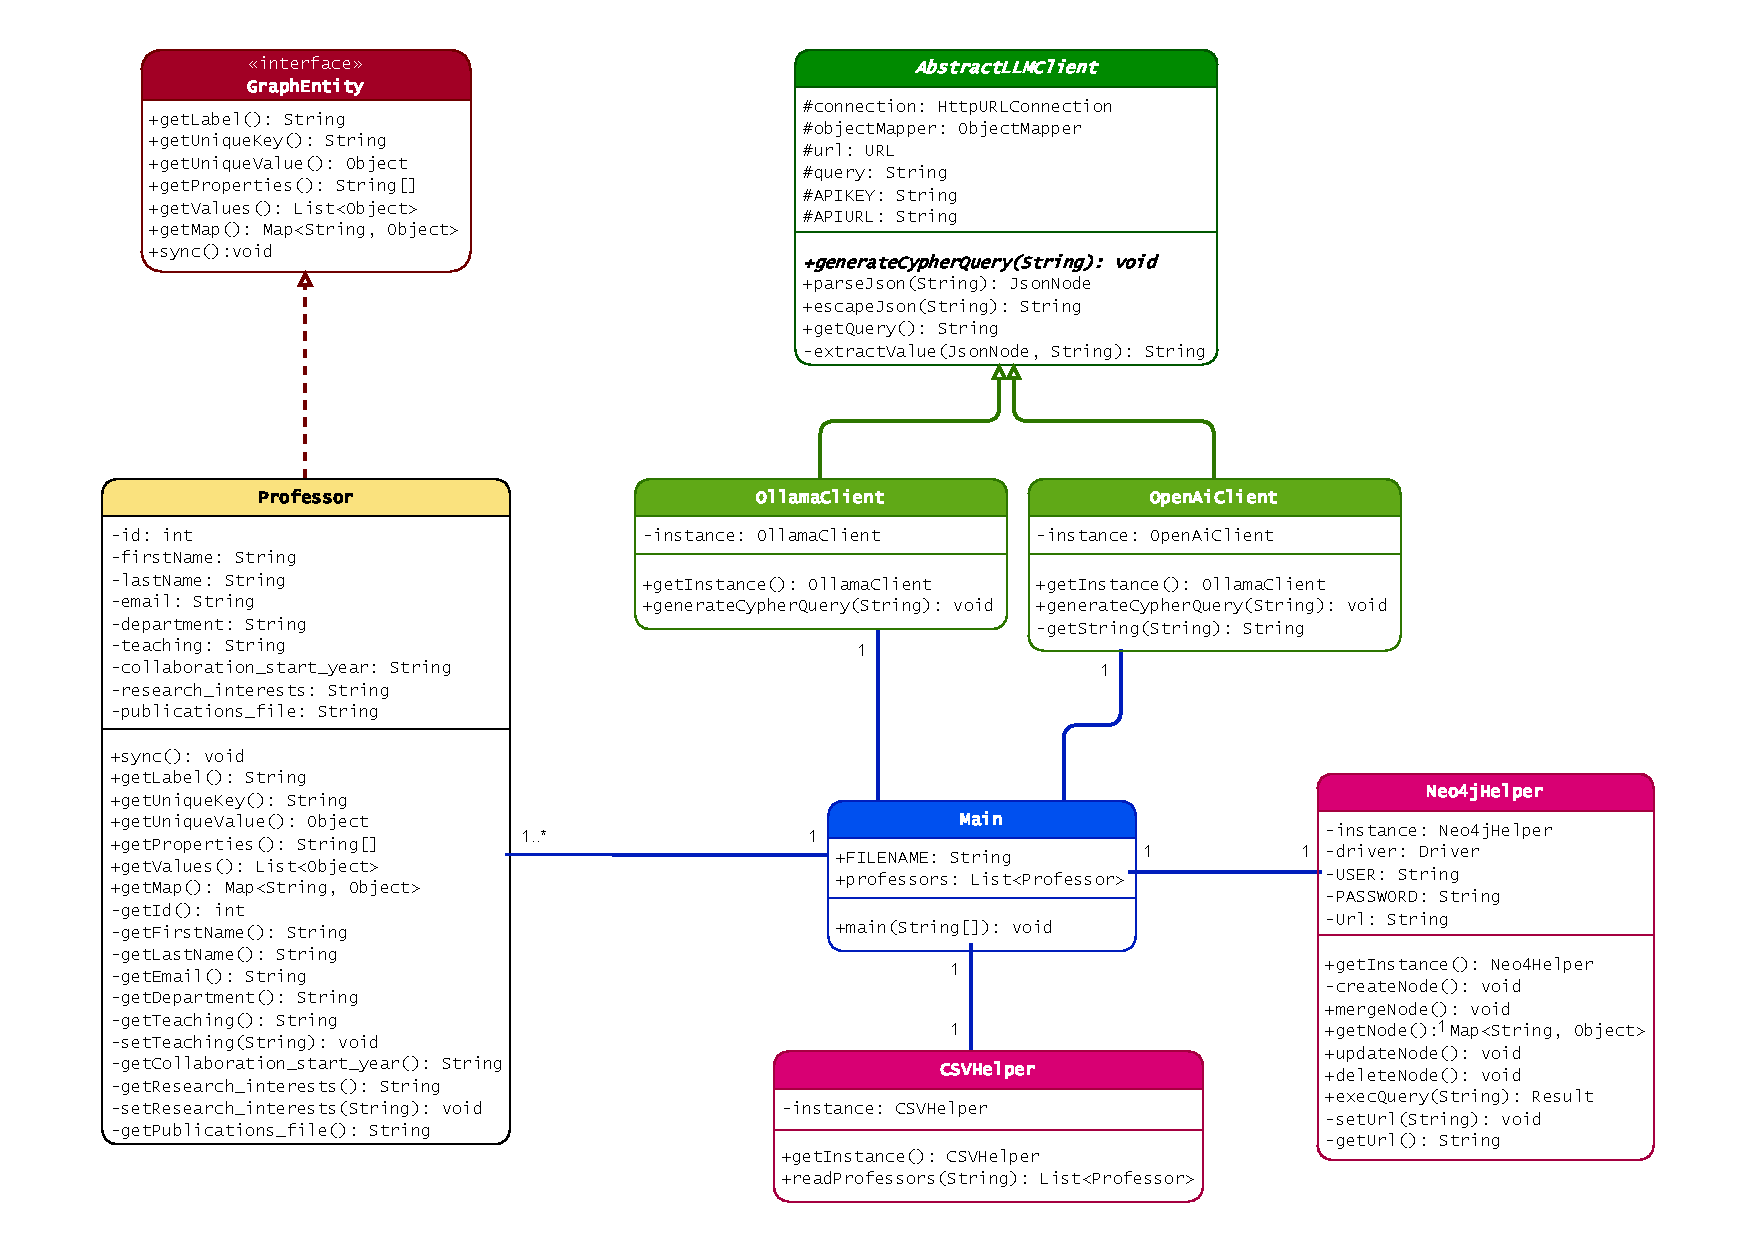
\includegraphics[width=\linewidth, height=0.72\textheight, keepaspectratio]{example_UML.pdf}
		\caption{High-level architecture}
	\end{figure}
\end{frame}

%=== FRAME: Figure + explanation side by side ==========================================
\begin{frame}{Class Diagram}
	\framesubtitle{Core entities}
	\begin{columns}[c]
		\begin{column}{0.58\textwidth}
			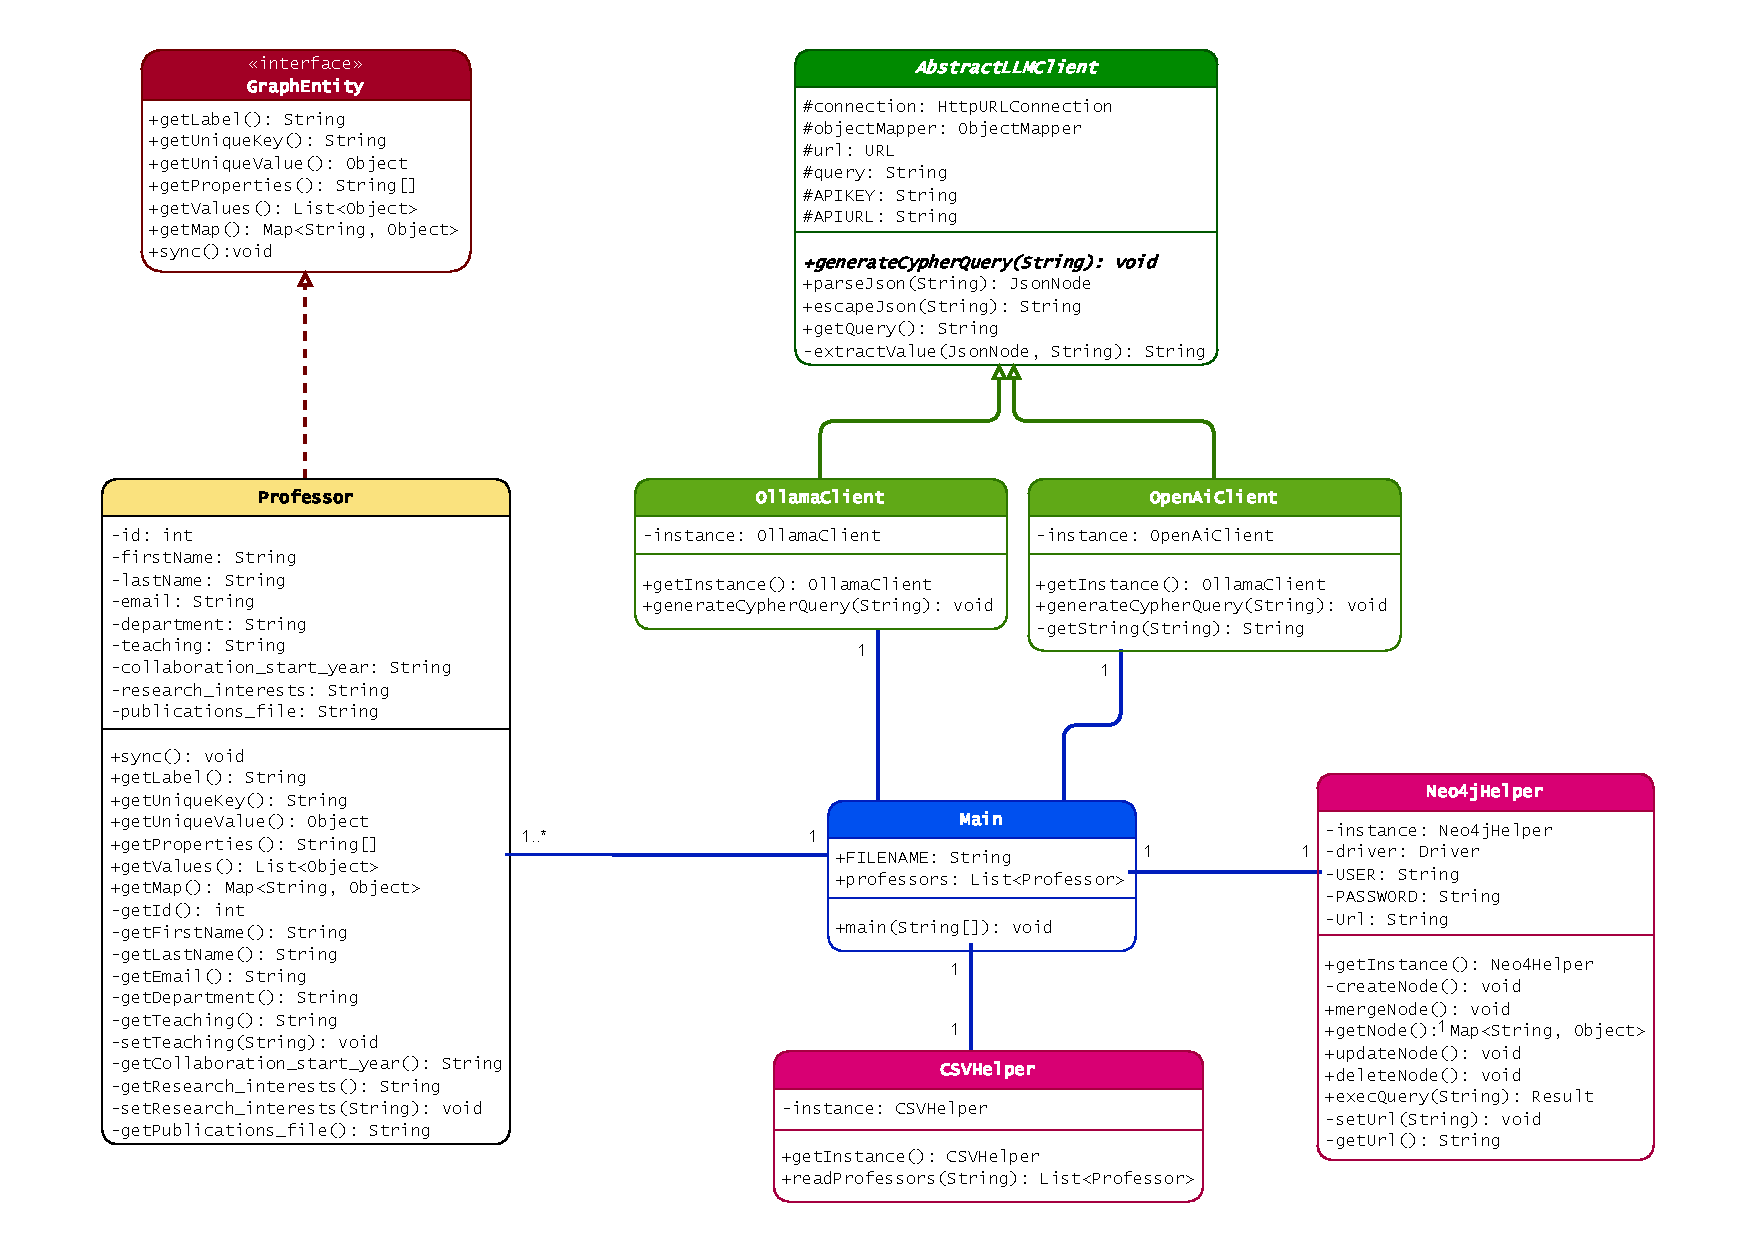
\includegraphics[width=\linewidth, height=0.7\textheight, keepaspectratio]{example_UML.pdf}
		\end{column}
		\begin{column}{0.38\textwidth}
			\begin{itemize}
				\item \textbf{User} --- base class for all roles
				\item \textbf{Association} --- has many members
				\item \textbf{Election} --- belongs to an association
			\end{itemize}
		\end{column}
	\end{columns}
\end{frame}

%=== FRAME: Simple diagram drawn in TikZ ===============================================
\begin{frame}{Request Workflow}
	\centering
	\begin{tikzpicture}[
		node distance=1.1cm and 1.2cm,
		box/.style={draw=brand, fill=lightbg, rounded corners, thick,
		            minimum width=2.4cm, minimum height=1cm, align=center, font=\small},
		arr/.style={-{Stealth[length=3mm]}, thick, accent},
	]
		\node[box] (a) {Secretary\\submits};
		\node[box, right=of a] (b) {Staff\\reviews};
		\node[box, right=of b, fill=enggreen!15, draw=enggreen] (c) {Approved};
		\node[box, below=of b, fill=lvlhigh!10, draw=lvlhigh] (d) {Needs\\changes};
		\draw[arr] (a) -- (b);
		\draw[arr] (b) -- (c);
		\draw[arr] (b) -- (d);
		\draw[arr] (d) -| (a);
	\end{tikzpicture}
\end{frame}

%----------------------------------------------------------------------------------------
\section{Implementation}
%----------------------------------------------------------------------------------------

%=== FRAME: Tech stack =================================================================
\begin{frame}{Technology Stack}
	\begin{columns}[T]
		\begin{column}{0.32\textwidth}
			\begin{block}{Mobile}
				\engb{Kotlin} \\ \engb{Room} \\ \engb{Retrofit}
			\end{block}
		\end{column}
		\begin{column}{0.32\textwidth}
			\begin{block}{Backend}
				\engb{Django} \\ \engb{PostgreSQL} \\ \engr{REST API}
			\end{block}
		\end{column}
		\begin{column}{0.32\textwidth}
			\begin{block}{DevOps}
				\engb{Docker Compose} \\ \engb{Git} / \engb{GitHub} \\ \engr{CI}
			\end{block}
		\end{column}
	\end{columns}
\end{frame}

%=== FRAME: Code snippet ===============================================================
% [fragile] is REQUIRED on any frame that contains \begin{lstlisting}
\begin{frame}[fragile]{API Example}
	\framesubtitle{\texttt{POST /api/requests/}}
	\begin{columns}[T]
		\begin{column}{0.5\textwidth}
			\textbf{Request}
\begin{lstlisting}[language=json]
{
  "title": "Python Workshop",
  "association_id": 12,
  "date": "2026-12-01",
  "capacity": 40
}
\end{lstlisting}
		\end{column}
		\begin{column}{0.46\textwidth}
			\textbf{Response} \engp{201 Created}
\begin{lstlisting}[language=json]
{
  "id": 87,
  "status": "pending"
}
\end{lstlisting}
		\end{column}
	\end{columns}
	% Keep \begin/\end{lstlisting} lines at column 0 — indentation would show up in the code.
\end{frame}

%----------------------------------------------------------------------------------------
\section{Project Management}
%----------------------------------------------------------------------------------------

%=== FRAME: Team =======================================================================
\begin{frame}{Team \& Responsibilities}
	\begin{columns}[T]
		\begin{column}{0.31\textwidth}
			\begin{block}{Zahra Mirzaei}
				\small\textbf{Android developer}\\[0.3em]
				App screens, voting, \engb{Room}, notifications
			\end{block}
		\end{column}
		\begin{column}{0.31\textwidth}
			\begin{block}{Amirmahdi Azizi}
				\small\textbf{Backend developer}\\[0.3em]
				\engb{PostgreSQL}, \engb{Django} API, auth, elections
			\end{block}
		\end{column}
		\begin{column}{0.31\textwidth}
			\begin{block}{Amirhossein Alian}
				\small\textbf{Integration}\\[0.3em]
				API contract, \engb{Docker}, admin panel, docs
			\end{block}
		\end{column}
	\end{columns}
\end{frame}

%=== FRAME: Timeline ===================================================================
% Edit the list in \foreach: {position/label/date}. Add or remove entries freely.
\begin{frame}{Timeline}
	\centering
	\begin{tikzpicture}[x=1.3cm]
		\draw[very thick, rulegray, -{Stealth[length=3mm]}] (0,0) -- (8.6,0);
		\foreach \x/\label/\date [count=\i] in {
			0/Proposal/Week 1,
			1.6/Requirements/Week 3,
			3.2/Design/Week 5,
			4.8/Implementation/Week 7--12,
			6.4/Testing/Week 13,
			8/Delivery/Week 15}{
			\fill[brand] (\x,0) circle (4pt);
			\ifodd\i
				\node[above=6pt, font=\small\bfseries, text=brand] at (\x,0) {\label};
				\node[below=6pt, font=\scriptsize, text=accent] at (\x,0) {\date};
			\else
				\node[below=6pt, font=\small\bfseries, text=brand] at (\x,0) {\label};
				\node[above=6pt, font=\scriptsize, text=accent] at (\x,0) {\date};
			\fi
		}
	\end{tikzpicture}
\end{frame}

%=== FRAME: Risk table =================================================================
\begin{frame}{Risks \& Mitigation}
	\rowcolors{2}{lightbg}{white}
	\begin{tabularx}{\linewidth}{L c c L}
		\toprule
		\rowcolor{brand}\textcolor{white}{\textbf{Risk}} &
		\textcolor{white}{\textbf{Probability}} &
		\textcolor{white}{\textbf{Impact}} &
		\textcolor{white}{\textbf{Mitigation}} \\
		\midrule
		Team member unavailable  & \med{Medium} & \high{High}  & Cross-training, shared docs \\
		API contract changes     & \high{High}  & \med{Medium} & Versioned API, early agreement \\
		Deadline pressure        & \med{Medium} & \med{Medium} & MVP first, stretch goals later \\
		\bottomrule
	\end{tabularx}
\end{frame}

%----------------------------------------------------------------------------------------
\section{Conclusion}
%----------------------------------------------------------------------------------------

%=== FRAME: Summary ====================================================================
\begin{frame}{Summary}
	\begin{enumerate}
		\item First key takeaway
		\item Second key takeaway
		\item What comes next
	\end{enumerate}
\end{frame}

%=== FRAME: Big centered message (demo / thanks / questions) ===========================
\begin{frame}[plain, noframenumbering]
	\centering
	\vfill
	{\Huge\bfseries\color{brand} \txtThanks}\\[1em]
	{\Large\color{accent} \txtQuestions}
	\vfill
\end{frame}

%----------------------------------------------------------------------------------------
%	BACKUP SLIDES (after the end; not counted in the page total)
%----------------------------------------------------------------------------------------
\appendix
\backupbegin

%=== FRAME: Backup =====================================================================
\begin{frame}{\txtBackup}
	Detailed tables, extra diagrams, answers to expected questions...
\end{frame}

\backupend

\end{document}
